%%%%%%%%%%%%%%%%%%%%%%%%%%%%%%%%%%%%%%%%%%%%%%%%%%%%
%%% Standalone Korean sample: Chapter 18
%%%%%%%%%%%%%%%%%%%%%%%%%%%%%%%%%%%%%%%%%%%%%%%%%%%%

\documentclass[output=book,
  colorlinks,citecolor=brown
]{langscibook}

\author{Brett Reynolds}
\title{언어의 풍경: Language Landscapes}
\subtitle{영어 교사를 위한 영어 구조 안내서[한국어판]}
% \ISBNdigital{}
% \ISBNhardcover{}
% \BookDOI{}
\typesetter{Brett Reynolds}
% \proofreader{}
% \lsCoverTitleSizes{51.5pt}{17pt}
\renewcommand{\lsSeries}{tbls}
%\newcommand{\lsSeriesTitle}{Textbooks in Language Sciences}
%\newcommand{\lsSeriesColor}{lsYellow}
\renewcommand{\lsSeriesNumber}{16}
\BackBody{언어는 외워야 할 목록이 아니라 탐구해야 할 풍경입니다.

좋은 현장 자연학자는 이름만 붙이지 않습니다. 무엇이 어떻게 행동하는지, 어디에 모이는지, 왜 달라지는지를 관찰합니다. 이 책은 영어를 같은 방식으로 읽도록 안내합니다. 규칙서가 영어가 어떠해야 한다고 말하는지가 아니라, 실제 화자가 무엇을 하는지에 주목하는 것입니다. 이론적 틀은 \textit{The Cambridge Grammar of the English Language}에 바탕을 두되, 접근하기 쉽게 단순화했습니다. 하지만 수준을 낮추지는 않았습니다.

각 장은 소리와 단어에서 구, 절, 담화로 나아가며, 분명한 영어 예문을 다른 언어의 단면과 함께 제시합니다. 각 장에서 같은 과정을 연습합니다. 패턴을 관찰하고, 증거로 검토하고, 어디에서 그 패턴이 무너지는지 보고, 그 무너짐이 무엇을 알려 주는지 묻는 과정입니다. 끝까지 읽고 나면, 교재를 평가하고, 학습자의 문장이 왜 조금 어색한지 설명하고, 질문을 받을 때 자신의 설명을 근거 있게 방어할 수 있는 실용적인 문법 지식을 갖게 될 것입니다.

교사 양성 과정에 있든 이미 교실에서 가르치고 있든, 얻는 것은 같습니다. 정당화할 수 없는 규칙에 기대는 일을 멈추고, 언어 체계를 스스로 볼 수 있게 됩니다.}

\usepackage{langsci-optional}
\usepackage{langsci-gb4e}
\usepackage{langsci-lgr}

% Load xeCJK for Japanese text (needed for マクドナルド etc)
\usepackage{xeCJK}
% Try common CJK serif fonts to match book's serif style
\IfFontExistsTF{Noto Serif CJK JP}{
  \setCJKmainfont{Noto Serif CJK JP}
  \setCJKsansfont{Noto Sans CJK JP}
  \setCJKmonofont{Noto Sans Mono CJK JP}
}{
  \IfFontExistsTF{Hiragino Mincho ProN}{
    \setCJKmainfont{Hiragino Mincho ProN}
    \setCJKsansfont{Hiragino Sans GB}
    \setCJKmonofont{Hiragino Sans GB}
  }{
    % Fallback - still prefer serif-style for main
    \setCJKmainfont{Arial Unicode MS}
    \setCJKsansfont{Arial Unicode MS}
    \setCJKmonofont{Arial Unicode MS}
  }
}
\usepackage{fontspec}
% Setting up Hindi font
\newfontfamily\hindifont{Noto Serif Devanagari}  % Replace [HindiFont] with your Hindi font

\usepackage{mdframed}
\usepackage{tcolorbox}
\tcbuselibrary{breakable}
\usepackage{tipa}
% contour and soul removed (no longer needed after underline cleanup)
\usepackage{ulem}  % retained for \xout{} in Ch 15 (ellipsis strikethrough)
\usepackage{langsci-tbls}
% Override tblsfilled: upstream uses frame-based fill that doesn't render
% reliably; use colback instead, and add breakable for page-spanning boxes
\RenewTColorBox{tblsfilled}{m O{black!12}}
  {
    enhanced,
    breakable,
    title = {#1},
    colback = #2,
    colframe = #2,
    boxrule = 0pt,
    boxsep = 0pt,
    toptitle = 5mm,
    top = 5mm,
    bottom = 5mm,
    left = 5mm,
    right = 5mm,
    sharp corners = all,
    coltitle = black,
    fonttitle = \normalfont\sffamily\bfseries\large,
  }
\usepackage{enumitem}
\usepackage{multicol}
\usepackage{forest}
\usepackage{graphicx}
\usepackage{wrapfig}
\usetikzlibrary{bending}
\usepackage{subcaption}
\usepackage{changepage}

% Fix header height warnings
\usepackage{geometry}
\geometry{head=27.2pt}

%\usepackage{fontspec}

%\setmainfont{Times New Roman} % Your main document font
%\newfontfamily\japanesefont{IPAMincho} % Japanese font
%\newfontfamily\hindifont[Script=Devanagari]{Lohit Devanagari} % Hindi font


\usepackage{listings}
\lstset{basicstyle=\ttfamily,tabsize=2,breaklines=true}

\usepackage{tikz}
\usetikzlibrary{tikzmark, positioning}

\usepackage{longtable}

\usepackage{dialogue}

\usepackage{paracol}

% mdframed already loaded above (line 28)

\usepackage{pifont}

\newfontfamily\ethiopic[Script=Ethiopic]{Abyssinica SIL}
\newfontfamily\persian[Script=Arabic]{Amiri}

% ==========================================================
%                  INDEX SETUP (REVISED)
% ==========================================================
% This setup uses a simpler definition to avoid conflicts.
% PLEASE REPLACE ALL OTHER INDEXING CODE WITH THIS BLOCK.

% 1. Load the package for indexing
\usepackage{imakeidx}

% 2. Create the three separate indexes + dummy output index
\makeindex[name=output, title=Output Index, columns=2]
\makeindex[name=sbj, title=Subject Index, columns=2, intoc]
\makeindex[name=lan, title=Language Index, columns=2, intoc]
\makeindex[name=aut, title=Author Index, columns=2, intoc]

% 3. Define simple, robust custom commands
% Using \renewcommand avoids conflicts with the langscibook class.
\renewcommand{\is}[1]{\index[sbj]{#1}}
\renewcommand{\il}[1]{\index[lan]{#1}}
\renewcommand{\ia}[1]{\index[aut]{#1}}
% ==========================================================

% csquotes for \enquote{} (smart quotation marks)
\usepackage{csquotes}

% Semantic typography macros
\newcommand{\mention}[1]{\textit{#1}}        % metalinguistic mention (word as object)
\newcommand{\mentionhead}[1]{⟨#1⟩}           % mention in headings (angle brackets)
\providecommand{\term}[1]{\textsc{#1}}       % technical term (small caps)

\usepackage{indentfirst}
\setlength{\parindent}{1em}

\IfFontExistsTF{Noto Serif CJK KR}{
  \setCJKmainfont{Noto Serif CJK KR}
  \setCJKsansfont{Noto Sans CJK KR}
  \setCJKmonofont{Noto Sans Mono CJK KR}
}{
  \IfFontExistsTF{Apple SD Gothic Neo}{
    \setCJKmainfont{Apple SD Gothic Neo}
    \setCJKsansfont{Apple SD Gothic Neo}
    \setCJKmonofont{Apple SD Gothic Neo}
  }{}
}
\xeCJKsetup{CJKspace=true}

\DeclareQuoteStyle{korean}{“}{”}{‘}{’}
\setquotestyle{korean}

\renewcommand{\contentsname}{목차}
\renewcommand{\figurename}{그림}
\renewcommand{\tablename}{표}
\renewcommand{\bibname}{참고문헌}
\renewcommand{\appendixname}{부록}
\renewcommand{\chapterformat}{제\thechapter{}장\autodot\enskip}
\renewcommand{\figureformat}{\figurename~\thefigure\autodot}
\renewcommand{\tableformat}{\tablename~\thetable\autodot}

\input{../localhyphenation.tex}
\addbibresource{../localbibliography.bib}

\graphicspath{{../}}

\begin{document}
\input{../localcommands.tex}
% Korean has no small-caps contrast; use Gothic/sans for technical terms.
\renewcommand{\term}[1]{\textsf{#1}}
\renewcommand{\mention}[1]{#1}
\renewcommand{\trans}[1]{`#1'}
\mainmatter
\setcounter{chapter}{17}
\chapter{종속화와 등위접속} \label{ch:subord-coord-ko}

\epigraph{If I were a cinnamon peeler\\
I would ride your bed\\
and leave the yellow bark dust\\
on your pillow.}{Michael Ondaatje, \enquote{The Cinnamon Peeler}}

\begin{tblsframedsymbol}{학습 목표}{bulb}
\begin{itemize}[noitemsep, leftmargin=*]
    \item \term{종속화}(\term{subordination})가 만드는 위계적 의존 관계와 \term{등위접속}(\term{coordination})이 만드는 동등한 지위의 결합을 구별할 수 있다.
    \item 복문 안에서 \term{모절}(\term{matrix clause}), \term{주절}(\term{main clause}), \term{종속절}(\term{subordinate clause})을 찾아 분석할 수 있다.
    \item \term{내용절}(\term{content clause}), \term{비교절}(\term{comparative clause}), \term{관계절}(\term{relative clause})이라는 주요 종속절 유형을 인식할 수 있다.
    \item \term{종속 접속사}(\term{subordinator})와 \term{등위접속사}(\term{coordinator})가 주요부가 아니라 구조적 표지로 기능한다는 점을 이해한다.
    \item 구의 등위접속과 절의 등위접속을 포함하여 등위 구조를 분석할 수 있다.
    \item 복문의 구조 관계를 판단하기 위한 진단 테스트를 적용할 수 있다.
    \item 종속화와 등위접속이 텍스트의 결속성을 만드는 데 어떻게 함께 작용하는지 이해한다.
    \item 이러한 구조가 통사적 인식을 기르는 데 어떤 교육적 가치가 있는지 이해한다.
\end{itemize}
\end{tblsframedsymbol}

\section{도입}

언어는 개별적인 생각만이 아니라 생각들 사이의 관계도 표현하게 해 줍니다. 이를 위한 두 가지 기본 방식은 \term{종속화}(\term{subordination})와 \term{등위접속}(\term{coordination})입니다. 둘은 서로 다른 일을 합니다. 종속화는 의존 관계의 위계를 만들고, 등위접속은 같은 지위의 요소를 결합합니다.

같은 기본 생각을 연결하는 다음 세 가지 방식을 보십시오.

\ea \label{ex:intro-ko}
    \ea \gll Kim left. Pat came.\\
        Kim 떠나다-PST Pat 오다-PST\\
    \glt \trans{킴은 떠났다. 팻은 왔다.} [분리]
    \ex \gll The fact {\ob}that Kim left{\cb} enabled Pat's arrival.\\
        DEF 사실 Sdr Kim 떠나다-PST 가능하게-하다-PST Pat-GEN 도착\\
    \glt \trans{킴이 떠났다는 사실이 팻의 도착을 가능하게 했다.} [종속]
    \ex \gll Kim left and Pat came.\\
        Kim 떠나다-PST and Pat 오다-PST\\
    \glt \trans{킴은 떠났고 팻은 왔다.} [등위]
    \z
\z
(\ref{ex:intro-ko}a)에는 두 개의 독립된 진술이 있습니다. (b)에서는 \mention{that Kim left}가 더 큰 구조 안에 들어가 있습니다. 그것은 주어 안에서 보충어로 기능합니다. (c)에서는 두 절이 같은 지위에 놓여 있습니다. 두 절은 동등한 것으로 제시되고, \mention{and}로 연결되어 있을 뿐입니다.

위계와 동등성의 이 대조는 문법에서 매우 중요합니다. 한 절을 다른 절에 종속시키면 의존 관계가 생깁니다. 한 절이 다른 절 안의 어떤 요소에 대한 보충어나 수식어로 기능합니다. 요소들을 등위접속하면, 다른 점에서는 차이가 있더라도 구조 안에서는 같은 지위를 가진다고 나타냅니다.

이 두 관계를 표시하는 도구는 많지 않습니다. 의존 관계에는 \mention{that}이나 \mention{whether} 같은 단어가 쓰이고, 동등성 관계에는 \mention{and}, \mention{or}, \mention{but} 같은 단어가 쓰입니다. 그러나 이 작은 단어들 덕분에 우리는 단순한 부분들로 복잡한 의미를 만들고, 생각들이 어떻게 연결되는지 보이며, 긴 추론의 흐름 속에서 독자를 안내할 수 있습니다. 이 요소들은 주요부가 아니라 문법적 관계를 표시하는 역할을 합니다.

이 장에서는 이 두 체계가 따로, 또 함께 어떻게 작동하는지 살펴봅니다. 종속화가 한 생각을 다른 생각 안에 넣어 의미의 층을 만드는 방식을 보겠습니다. 등위접속이 구조적 단순성을 유지하면서도 복잡한 생각을 만들게 해 주는 방식도 보겠습니다. 마지막으로 두 체계가 서로를 보완하여 거의 어떤 생각의 관계도 표현할 수 있게 해 주는 유연성을 확인하겠습니다.

\section{종속화}\label{sec:subordination-ko}

의사소통을 할 때 우리는 생각들 사이의 복잡한 관계를 자주 표현해야 합니다. 어떤 생각이 다른 생각에 의존하기도 하고, 어떤 생각이 다른 생각을 수식하거나 설명하기도 합니다. 여기서 종속화가 중요해집니다. \term{종속화}란 한 절을 다른 구조 안의 \term{의존부}(\term{dependent})로 만드는 문법적 과정입니다.

\term{종속절}(\term{subordinate clause})을 포함하는 절은 \term{모절}(\term{matrix clause})이라고 부릅니다. 반대로 자신을 포함하는 모절이 없는 절은 \term{주절}(\term{main clause})이라고 부릅니다. 다음 예가 보여 주듯이, 한 절은 동시에 주절이면서 모절일 수 있습니다.

\ea \label{ex:sub-basic-ko}
    \ea \gll Kim left early.\\
        Kim 떠나다-PST 일찍\\
    \glt \trans{킴은 일찍 떠났다.} [주절]
    \ex \gll She thinks {[}that Kim left early{]}.\\
        she 생각하다-PRS {[}Sdr Kim 떠나다-PST 일찍{]}\\
    \glt \trans{그녀는 킴이 일찍 떠났다고 생각한다.} [종속]
    \ex \gll {[}She thinks that Kim left early{]}.\\
        {[}she 생각하다-PRS Sdr Kim 떠나다-PST 일찍{]}\\
    \glt \trans{그녀는 킴이 일찍 떠났다고 생각한다.} [주절/모절]
    \z
\z
(\ref{ex:sub-basic-ko}a)는 단순한 주절입니다. (b)에서는 같은 절이 종속절이 되었습니다. 즉 (c)의 모절 안에 있는 의존부가 되었습니다. 그리고 (c)의 모절은 동시에 주절입니다.

이 패턴은 더 확장될 수 있습니다. (\ref{ex:sub-basic2-ko})에서 (\ref{ex:sub-basic-ko}b)의 절은 주절에서 종속절로 바뀌었지만, 여전히 \mention{that Kim left}에 대한 모절입니다. 다시 말해 한 절은 주절이면서 모절일 수 있을 뿐 아니라, 종속절이면서 모절일 수도 있습니다.

\ea\label{ex:sub-basic2-ko}
\gll I heard {\ob}that she thinks {\ob}that Kim left early{\cb}{\cb}.\\
    I 듣다-PST Sdr she 생각하다-PRS Sdr Kim 떠나다-PST 일찍\\
\glt \trans{나는 그녀가 킴이 일찍 떠났다고 생각한다고 들었다.} [종속]
\z

하지만 어떤 절도 동시에 \term{주절}과 \term{종속절}일 수는 없습니다. \term{모절}과 \term{종속절}은 관계를 나타내는 용어입니다. 한 절이 다른 절에 대해 어떤 위치에 있는지를 말합니다. 반면 \term{주절}은 통사적 유형을 가리킵니다. 그리고 주절의 구조가 여러 종속절 유형에서 항상 그대로 보존되는 것은 아닙니다.

\subsection{종속절의 유형}

영어에는 주요한 정형 종속절이 세 종류 있습니다.\footnote{\textit{CGEL}은 정형 종속절과 비정형 종속절을 구별하고, 그 안에서도 여러 하위 유형을 세웁니다. 여기서는 다루지 않습니다.} \term{내용절}(\term{content clause}), \term{비교절}(\term{comparative clause}), \term{관계절}(\term{relative clause})입니다. 차례로 살펴봅시다.

\ea \label{ex:sub-types-ko}
    \ea \gll I doubt that we ordered enough books.\\
        I 의심하다-PRS Sdr we 주문하다-PST 충분한 책-PL\\
    \glt \trans{나는 우리가 충분한 책을 주문했는지 의심스럽다.} [내용]
    \ex \gll More books arrived than we had ordered.\\
        더-많은 책-PL 도착하다-PST than we 주문하다-PST\\
    \glt \trans{우리가 주문했던 것보다 더 많은 책이 도착했다.} [비교]
    \ex \gll The books that we ordered arrived.\\
        DEF 책-PL Rel we 주문하다-PST 도착하다-PST\\
    \glt \trans{우리가 주문한 책들이 도착했다.} [관계]
    \z
\z
내용절은 기본적인 경우입니다. 관계절이나 비교절이 가지는 특별한 통사적 성질을 가지지 않습니다. 관계절은 다음 장의 주제이므로, 여기서는 먼저 내용절을 보고 그다음 비교절을 다루겠습니다.

\subsubsection{내용절}

내용절에는 크게 두 종류가 있습니다. (\ref{ex:content-types-ko})에서 보듯이 평서절과 의문절입니다.\footnote{\textit{CGEL}은 감탄 내용절도 다루지만, 매우 드뭅니다.}

\ea \label{ex:content-types-ko}
    \ea \gll She said that it was genuine.\\
        she 말하다-PST Sdr it 이다-PST 진짜\\
    \glt \trans{그녀는 그것이 진짜라고 말했다.} [평서]
    \ex \gll She asked whether it was genuine.\\
        she 묻다-PST whether it 이다-PST 진짜\\
    \glt \trans{그녀는 그것이 진짜인지 물었다.} [기본 의문]
    \ex \gll She asked what made it genuine.\\
        she 묻다-PST what 만들다-PST it 진짜\\
    \glt \trans{그녀는 무엇이 그것을 진짜로 만드는지 물었다.} [초점화 의문]
    \z
\z
(\ref{ex:content-types-ko}a와 b)의 \mention{that}과 \mention{whether}는 중요한 일을 합니다. 각각의 절이 종속되어 있음을 표시합니다. 여기서 새롭지만 매우 작은 범주인 \term{종속 접속사}(\term{subordinator}, Sdr)가 등장합니다. 이 범주의 주요 구성원은 \mention{that}과 \mention{whether}, 그리고 \enquote{whether}의 뜻을 가진 \mention{if}입니다. 조건을 나타내는 \mention{if}가 아닙니다. 한국어 문법에서 \enquote{접속사}라는 말은 넓게 쓰일 수 있지만, 여기의 \term{종속 접속사}는 더 좁은 통사 범주입니다. 명사에는 NP가 있고 동사에는 VP가 있지만, 종속 접속사에는 SdrP가 없습니다. 종속 접속사는 구를 투사하지 않고, 오직 그 절이 더 큰 구조와 어떤 관계를 맺는지 표시합니다. 나무 구조는 그림~\ref{fig:sub-tree-sub-ko}에 보입니다. (삼각형은 구조 일부가 생략되었음을 나타냅니다. 6장을 보십시오.)

\begin{figure}
    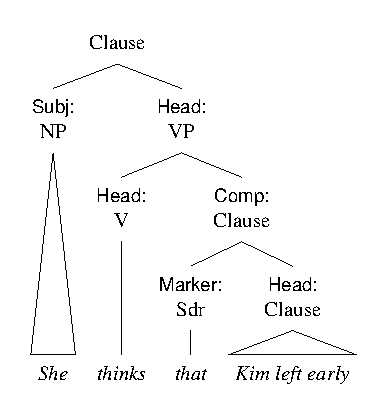
\includegraphics[width=0.55\linewidth]{figures/she thinks that kim left.pdf}
    \caption{종속화를 보여 주는 통사 나무: \mention{She thinks that Kim left early}에서 \mention{that Kim left early}가 보충어로 기능한다}\label{fig:sub-tree-sub-ko}
\end{figure}

종속 구조에서 \mention{that}이 표지로 나타난다는 점에 주목하십시오. \mention{that}은 자기 자신의 구를 투사하지 않고, 단지 종속절의 시작을 표시합니다. \term{표지어}(\term{marker}, Mk)는 주요부가 더 큰 구조와 문법적으로 어떻게 관련되는지를 표시하는 의존부의 한 종류입니다.

내용절은 더 큰 구조 안에서 여러 방식으로 기능할 수 있습니다.

\ea \label{ex:content-funcs-ko}
    \ea \gll I suspect {\ob}that he left{\cb}.\\
        I 의심하다-PRS Sdr he 떠나다-PST\\
    \glt \trans{나는 그가 떠났다고 짐작한다.} [VP 안]
    \ex \gll The fact {\ob}that he left{\cb} is clear.\\
        DEF 사실 Sdr he 떠나다-PST 이다-PRS 분명한\\
    \glt \trans{그가 떠났다는 사실은 분명하다.} [NP 안]
    \ex \gll I'm glad {\ob}that he left{\cb}.\\
        I-이다 기쁜 Sdr he 떠나다-PST\\
    \glt \trans{그가 떠나서 나는 기쁘다.} [AdjP 안]
    \ex \gll We can proceed provided {\ob}that he left{\cb}.\\
        we 할-수-있다-PRS 진행하다 provided Sdr he 떠나다-PST\\
    \glt \trans{그가 떠났다면 우리는 진행할 수 있다.} [PP 안]
    \ex \gll Whether or not he left is unclear.\\
        whether or not he 떠나다-PST 이다-PRS 불분명한\\
    \glt \trans{그가 떠났는지 아닌지는 분명하지 않다.} [주어]
    \ex \gll It's unclear whether or not he left.\\
        it-이다 불분명한 whether or not he 떠나다-PST\\
    \glt \trans{그가 떠났는지 아닌지는 분명하지 않다.} [외치 주어]
    \z
\z

평서 내용절에서는 표지어, 곧 종속 접속사 \mention{that}이 그 절의 기능에 따라 필수일 수도 있고, 선택적일 수도 있고, 허용되지 않을 수도 있습니다.
\ea\label{ex:marker-need-ko}
    \ea \gll That Kim left surprised no one.\\
        Sdr Kim 떠나다-PST 놀라게-하다-PST 아무도-아님\\
    \glt \trans{킴이 떠났다는 사실은 아무도 놀라게 하지 않았다.} [필수]
    \ex \gll I know that Kim left.\\
        I 알다-PRS Sdr Kim 떠나다-PST\\
    \glt \trans{나는 킴이 떠났다는 것을 안다.} [선택]
    \ex \gll *We left before that Kim arrived.\\
        *we 떠나다-PST before Sdr Kim 도착하다-PST\\
    \glt \trans{의도한 뜻: 우리는 킴이 도착하기 전에 떠났다. 영어에서는 여기서 \mention{that}을 쓸 수 없다.} [*; 불가]
\z
\z
(\ref{ex:marker-need-ko}a) 같은 주어절에서는 표지어가 항상 필요합니다. 보충어로 기능할 때 평서절은 대개 (b)처럼 표지어가 있어도 되고 없어도 됩니다. 중요한 예외는 (c)처럼 PP 안에서 보충어로 기능하는 경우입니다.

\label{sec:sub-interrog-ko}

의문 내용절은 흥미롭습니다. 주절 의문절과 통사적으로 다르기 때문입니다. 주절의 기본 의문절은 \mention{Did she accept?}처럼 주어와 조동사가 도치되는 것으로 알아볼 수 있습니다. 반면 종속절 버전은 \mention{whether}나 \mention{if}로 의문임을 표시합니다.

\ea 기본 의문절\label{ex:int-sub-ko}
    \ea \gll Did she accept?\\
        AUX she 받아들이다\\
    \glt \trans{그녀는 받아들였는가?} [주절, 도치]
    \ex \gll I wonder {\ob}whether she accepted{\cb}.\\
        I 궁금해하다-PRS whether she 받아들이다-PST\\
    \glt \trans{나는 그녀가 받아들였는지 궁금하다.} [종속]
    \z
\z
\ea 초점화 의문절
    \ea \gll How did we get here?\\
        how AUX we 오다 여기로\\
    \glt \trans{우리는 어떻게 여기까지 왔는가?} [주절, 도치]
    \ex \gll I wonder {\ob}how we got here{\cb}.\\
        I 궁금해하다-PRS how we 오다-PST 여기로\\
    \glt \trans{나는 우리가 어떻게 여기까지 왔는지 궁금하다.} [종속]
    \z
\z
이 점은 영어 학습자에게 어렵습니다. 초급 학습자는 대개 아무것도 도치하지 않아 주절 의문절을 잘못 만들고, 더 경험 있는 학습자는 도치를 배운 뒤 그것을 어디에나 적용하여 종속 의문절을 잘못 구성합니다. 이 차이를 편하게 다루려면 꽤 높은 수준의 숙달이 필요합니다.

그렇지만 주절 의문절과 종속 의문절의 구조적 차이는 조금씩 약해지고 있습니다. 도치가 천천히 확장되고 있기 때문입니다. 글에서 도치된 의문 내용절을 보는 일은 아직 드물지만, (\ref{ex:non-inverted-interrogative-ko}) 같은 예는 말에서는 꽤 흔해지고 있습니다. 몇백 년 뒤에는 모든 의문절에서 도치가 표준이 되고 표지어가 선택적이 될지도 모릅니다. 저는 기다릴 생각이 없습니다.

\ea\label{ex:non-inverted-interrogative-ko}
\gll We need a story of {\ob}how did we get here{\cb}.\\
    we 필요로-하다-PRS a 이야기 of how AUX we 오다 여기로\\
\glt \trans{우리는 어떻게 여기까지 왔는지에 관한 이야기가 필요하다.}
\z
하지만 현재로서는 기본 의문 내용절에서 \mention{whether}나 \mention{if} 같은 표지어가 항상 필요합니다. 그렇지 않으면 대부분의 경우 표지어 없는 평서절과 구별할 수 없게 됩니다.

\subsubsection*{mandative 구문}

종속 구문의 특수한 하위 유형으로 \term{mandative 구문}이 있습니다. 이 구문은 요구나 필요성을 나타내는 술어와 함께 나타납니다.

\ea \label{ex:mandative-ko}
    \ea \gll It is essential {\ob}that he be there{\cb}.\\
        it 이다-PRS 필수적인 Sdr he 있다-PLAIN 거기에\\
    \glt \trans{그가 거기에 있는 것이 필수적이다.} [현재 가정법]
    \ex \gll It is essential {\ob}that he should be there{\cb}.\\
        it 이다-PRS 필수적인 Sdr he should 있다 거기에\\
    \glt \trans{그가 거기에 있어야 한다는 것이 필수적이다.} [should]
    \ex \gll It is essential {\ob}that he is there{\cb}.\\
        it 이다-PRS 필수적인 Sdr he 있다-PRS 거기에\\
    \glt \trans{그가 거기에 있다는 것이 필수적이다.} [직설법]
    \z
\z
\term{현재 가정법}(\term{present subjunctive}) 변형에서는 동사의 원형이 쓰입니다. 여기서 \enquote{가정법}이라는 말은 반사실을 뜻한다는 의미가 아닙니다. 영어 \mention{that he be there}에서 중요한 것은 요구나 필요성의 맥락에서 \mention{be}라는 원형이 나타난다는 점입니다. \mention{should}형은 적어도 예전에는 영국 영어에서 더 흔했습니다. 미국 영어는 현재 가정법을 선호하는 경향이 있습니다. \term{직설법}(\term{indicative}) 변형에서는 보통의 시제 굴절형이 쓰입니다.

이는 종속절 안의 변이가 미묘한 의미 차이와 지역적 선호를 보일 수 있음을 잘 보여 줍니다. 교육적으로는 직설법 형태가 특히 비격식 맥락에서 더 흔해지고 있지만, 공식적인 글에서는 현재 가정법이 여전히 표준이라는 점을 지적할 만합니다.

\begin{tblsframedsymbol}{이해 확인: 모절과 종속절}{test}
구조 관계를 찾아보십시오.
\begin{itemize}[noitemsep, leftmargin=*]
    \item \mention{I know that she thinks that he left}에서 주절, 모절, 종속절을 찾으십시오.
    \item \mention{She asked whether he left}에는 도치가 없지만 \mention{Did he leave?}에는 도치가 있는 이유를 설명하십시오.
    \item mandative 구문을 찾으십시오: \mention{It's important that he be careful}과 \mention{It's important that he is careful}.
\end{itemize}
이러한 구조 관계를 이해하면 의미가 통사 구조에서 어떻게 생기는지 더 잘 볼 수 있습니다.
\end{tblsframedsymbol}

\subsection{비교절}

정형 종속절의 두 번째 주요 유형은 비교절입니다. 비교절은 (\ref{ex:comparative-intro-ko})처럼 비교를 완성하는 절입니다.

\ea \label{ex:comparative-intro-ko}
    \ea \gll The ice was thicker than {\ob}we expected{\cb}.\\
        DEF 얼음 이다-PST 더-두꺼운 than we 예상하다-PST\\
    \glt \trans{얼음은 우리가 예상했던 것보다 더 두꺼웠다.}
    \ex \gll She writes faster than {\ob}she speaks{\cb}.\\
        she 쓰다-PRS 더-빠르게 than she 말하다-PRS\\
    \glt \trans{그녀는 말하는 것보다 더 빠르게 쓴다.}
    \ex \gll It doesn't cost as much as {\ob}I'd thought{\cb}.\\
        it NEG 들다-PRS as 많이 as I-생각하다-PST\\
    \glt \trans{그것은 내가 생각했던 것만큼 비용이 많이 들지 않는다.}
    \z
\z
비교절을 내용절과 구별하는 것은 비교절에 생략이 들어 있다는 점입니다. 문맥에서 회복할 수 있는 요소가 빠집니다. (\ref{ex:comparative-ellipsis-ko})에서 \dots 는 생략을 나타냅니다.\footnote{앞 장에서 공백을 도입했습니다. 공백은 나무 안에 있는 구조적 위치입니다. 반면 생략은 문맥에서 의미적으로 회복할 수 있는 자료이지만, 통사적 요소로 존재하지는 않습니다.}

\ea \label{ex:comparative-ellipsis-ko}
    \ea \gll Kim read more books than {\ob}Pat read \dots{\cb}.\\
        Kim 읽다-PST 더-많은 책-PL than Pat 읽다-PST \dots\\
    \glt \trans{킴은 팻이 읽은 것보다 더 많은 책을 읽었다.}
    \ex \gll Kim read more books than {\ob}Pat did \dots{\cb}.\\
        Kim 읽다-PST 더-많은 책-PL than Pat AUX.PST \dots\\
    \glt \trans{킴은 팻보다 더 많은 책을 읽었다.}
    \ex \gll Kim read more books than {\ob}Pat{\cb}.\\
        Kim 읽다-PST 더-많은 책-PL than Pat\\
    \glt \trans{킴은 팻보다 더 많은 책을 읽었다.}
    \z
\z

처음 두 변형은 생략을 보입니다. (b)에서는 \mention{read}를 반복하는 대신 VP 대용 형식인 \mention{did}가 쓰입니다. 세 번째 (c)에서 \mention{Pat}은 절의 보충어가 아니라 NP 보충어입니다. 세 문장은 기본적으로 같은 뜻입니다.

대부분의 생략과 달리, 비교절에서는 생략된 정보를 명시하면 비문이 됩니다. 예를 들어 *\mention{Kim read more books than Pat read 20 books}나 *\mention{It's not as deep as it is 20 cm wide}라고 할 수 없습니다. 생략은 이 절 유형의 핵심 부분입니다. 비교절의 구조는 그림~\ref{fig:comp-tree-ko}에 보입니다.

\begin{figure}
    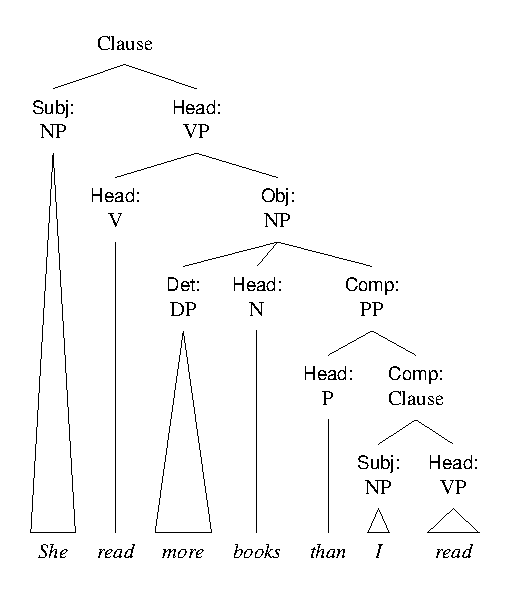
\includegraphics[width=0.7\linewidth]{figures/she read more books than I read.pdf}
    \caption{생략을 포함하는 비교절을 보여 주는 통사 나무}\label{fig:comp-tree-ko}
\end{figure}

비교절은 비교의 종류에 따라 \mention{than}이나 \mention{as}를 가진 PP 안에서 보충어로 기능합니다.

\ea \label{ex:comp-markers-ko}
    \ea \gll Kim is taller than {\ob}Pat is{\cb}.\\
        Kim 이다-PRS 더-키-큰 than Pat 이다-PRS\\
    \glt \trans{킴은 팻보다 키가 크다.} [불등]
    \ex \gll Kim is as tall as {\ob}Pat is{\cb}.\\
        Kim 이다-PRS as 키-큰 as Pat 이다-PRS\\
\glt \trans{킴은 팻만큼 키가 크다.} [동등\footnote{여기서 \enquote{\emph{동등}}이라는 말은 조금 오해를 부를 수 있습니다. 이 예는 킴이 적어도 팻만큼 키가 크다는 뜻이며, 킴이 더 클 수도 있습니다.}]
    \z
\z
(\ref{ex:comp-markers-ko}a)의 \mention{than}은 불등을 나타내고, (b)의 \mention{as}는 동등을 표시합니다. 첫 번째 \mention{as}는 부사입니다. \mention{as tall}이라는 AdjP가 있고, 그 안에서 \mention{as}는 수식어로 기능합니다. 두 번째 \mention{as}는 전치사입니다.

영어 학습자에게 비교절에는 몇 가지 어려움이 있습니다.
\begin{itemize}[noitemsep]
    \item 무엇을 언제 얼마나 생략할 수 있는지 이해하기.
    \item 동등과 불등의 서로 다른 유형 익히기.
    \item 여러 요소가 걸린 복잡한 비교 다루기.
\end{itemize}

좋은 소식은 비교절이 꽤 규칙적인 패턴을 따른다는 것입니다. 학습자는 더 복잡한 구조로 가기 전에 \mention{taller than} `...보다 키가 큰'이나 \mention{as tall as} `적어도 ...만큼 키가 큰' 같은 기본 형식을 익힐 수 있습니다.

\section{등위접속}\label{sec:coordination-ko}

종속화가 절들 사이에 의존 관계를 만드는 반면, \term{등위접속}은 같은 통사적 지위를 가진 요소들을 결합합니다. 이 체계의 중심에는 \term{등위접속사}(\term{coordinator}, Crd)라고 부르는 작고 닫힌 단어 부류가 있습니다. 주요 구성원은 \mention{and}, \mention{or}, \mention{but}입니다. 세 가지를 열거하는 데에도 세 가지가 모두 필요합니다. 종속 접속사와 마찬가지로 등위접속사도 표지어로 기능합니다.

여기서 \term{등위접속}은 단순히 생각이 자연스럽게 이어진다는 뜻이 아닙니다. 한국어의 \enquote{연결}이나 \enquote{접속}이라는 말은 담화의 흐름까지 넓게 떠올리게 할 수 있지만, 이 장에서 필요한 것은 구조적 관계입니다. 둘 이상의 요소가 같은 통사적 지위를 가지며, 어느 것도 전체의 주요부가 아닙니다. 이 점을 놓치면 등위접속을 단순한 목록이나 담화상의 이어짐으로 잘못 이해하기 쉽습니다.

다음 예를 보십시오.

\ea \label{ex:coord-basic-ko}
    \ea \gll {\ob}Jane is a good teacher{\cb} {\ob}and her students really like her{\cb}.\\
        Jane 이다-PRS a 좋은 교사 and her 학생-PL 정말 좋아하다-PRS her\\
    \glt \trans{제인은 좋은 교사이고 학생들은 그녀를 정말 좋아한다.}
    \ex \gll They offered us a choice of {\ob}red wine{\cb}, {\ob}white wine{\cb}, {\ob}or beer{\cb}.\\
        they 제안하다-PST us a 선택 of 빨간 와인 흰 와인 or 맥주\\
    \glt \trans{그들은 우리에게 레드 와인, 화이트 와인 또는 맥주라는 선택지를 제시했다.}
    \ex \gll Her assistant is {\ob}very young{\cb} {\ob}but a quick learner{\cb}.\\
        her 조수 이다-PRS 매우 어린 but a 빠른 학습자\\
    \glt \trans{그녀의 조수는 매우 어리지만 배우는 속도가 빠르다.}
    \z
\z
이 예들에서 해당 요소들은 \term{등위 요소}(\term{coordinate})로 기능합니다. 이 기능은 (\ref{ex:coord-basic-ko}a)처럼 절로 실현될 수도 있고, (b)처럼 NP나 다른 구로 실현될 수도 있으며, 더 드물게는 (c)의 AdjP와 NP처럼 범주가 섞여 실현될 수도 있습니다. 등위접속사는 보통 서로 다른 관계를 표현합니다. \mention{and}는 추가, \mention{or}는 선택, \mention{but}은 대조를 나타냅니다.

등위접속이 앞에서 본 구조와 다른 점은 주요부가 없다는 것입니다. 어떤 등위 요소도 전체 구조의 주요부가 아닙니다. 이 주요부 없음은 단순한 테스트에서 보입니다. 많은 경우 등위접속 전체를 등위 요소 가운데 하나로 바꿀 수 있습니다.

\ea \label{ex:coord-replace-ko}
    \ea \gll Her assistant is very young.\\
        her 조수 이다-PRS 매우 어린\\
    \glt \trans{그녀의 조수는 매우 어리다.}
    \ex \gll Her assistant is a quick learner.\\
        her 조수 이다-PRS a 빠른 학습자\\
    \glt \trans{그녀의 조수는 배우는 속도가 빠르다.}
    \z
\z
(\ref{ex:coord-replace-ko}a)와 (b)는 둘 다 (\ref{ex:coord-basic-ko}c)의 문법적인 대체 표현입니다. 이는 \mention{very young}처럼 주요부가 있는 구조와 매우 다릅니다. 그런 경우 주요부만은 쓸 수 있지만(\mention{she's young}), 의존부만은 쓸 수 없습니다(*\mention{she's very}). 등위접속의 구조는 그림~\ref{fig:coord-basic-ko}에 보입니다.

\begin{figure}
    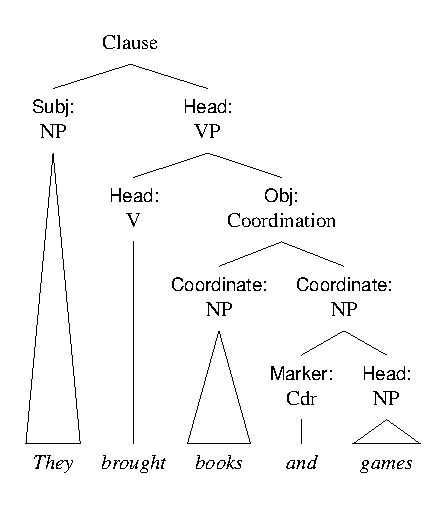
\includegraphics[width=0.65\linewidth]{figures/the brought books and games.pdf}
    \caption{표지어를 가진 기본 등위접속: \mention{They brought books and games}}\label{fig:coord-basic-ko}
\end{figure}

\subsection{등위접속의 성질}

세 가지 중요한 성질이 등위접속을 다른 구조와 구별합니다.

등위 요소의 수에는 문법적 제한이 없습니다. \mention{but}은 예외입니다.

\ea \label{ex:coord-multiple-ko}
\gll Nothing noble, sublime, profound, delicate, tasteful or even decent can find a place.\\
    아무것도 고귀한 숭고한 깊은 섬세한 품위-있는 or 심지어 괜찮은 할-수-있다-PRS 찾다 a 자리\\
\glt \trans{고귀하고, 숭고하고, 깊고, 섬세하고, 품위 있고, 심지어 괜찮은 것조차 자리를 찾을 수 없다.}
\z

등위 요소들은 기능적으로 비슷해야 합니다. 단독으로 쓰였을 때 같은 기능을 할 수 있어야 합니다.

\ea \label{ex:coordinate-function-ko}
    \ea \gll I'll be back next week or at the end of the month.\\
        I-FUT 돌아오다 다음 주 or at DEF 끝 of DEF 달\\
    \glt \trans{나는 다음 주나 월말에 돌아올 것이다.} [시간 부가어]
    \ex \gll *We're leaving Rome and next week.\\
        *we-PRS 떠나다 Rome and 다음 주\\
    \glt \trans{의도한 구조는 영어에서 어색하다. \mention{Rome}은 목적어이지만 \mention{next week}는 부가어이다.} [*; 목적어와 부가어]
    \z
\z

확장된 등위 요소, 즉 등위접속사를 포함하는 등위 요소는 앞쪽으로 이동할 수 없습니다.

\ea \label{ex:coord-front-ko}
    \ea \gll They attended but they aren't members.\\
        they 참석하다-PST but they NEG-이다-PRS 회원-PL\\
    \glt \trans{그들은 참석했지만 회원은 아니다.}
    \ex \gll *But they aren't members, they attended.\\
        *but they NEG-이다-PRS 회원-PL they 참석하다-PST\\
    \glt \trans{의도한 뜻: 그들은 참석했지만 회원은 아니다. 영어에서는 \mention{but}을 가진 확장 등위 요소를 이렇게 앞으로 보낼 수 없다.} [*]
    \z
\z

\subsection{문장 앞 등위접속사에 대한 말}

\mention{and}나 \mention{but} 같은 등위접속사로 문장을 시작하지 말라는 규범적 조언이 있습니다. 그러나 이 금지는 영어 문법이나 실제 사용에 근거가 없습니다. 문장 앞 등위접속사는 영어의 역사 전체에서 능숙한 글쓴이들이 사용해 왔습니다. 이 책에서도, 이 장과 다른 장에서도 많은 예를 찾을 수 있습니다. 다만 문장 앞 등위접속사는 그 문장을 앞 문장과 좁은 의미의 등위접속으로 묶을 수 없습니다. (\ref{ex:coord-front-ko})의 전치 제한을 떠올리십시오. 대신 그것은 \term{담화 연결 표현}(\term{discourse connector})으로 기능하여 새 문장이 앞 내용과 어떻게 관련되는지를 표시할 수 있습니다.

이 점은 한국어 독자에게 특히 혼동되기 쉽습니다. 담화 연결 표현은 글의 흐름을 이어 줍니다. 반면 이 장에서 말하는 등위접속은 하나의 통사 구조 안에서 같은 지위의 요소들을 결합하는 것입니다. 진짜 제한은 문체적 제한뿐입니다. 어떤 도구든 그렇듯 문장 앞 등위접속사도 너무 자주 쓰면 단조로워질 수 있습니다. 신중하게 쓰면 담화의 흐름을 관리하고 텍스트 안의 관계를 표시하는 유용한 수단입니다.

\subsection{등위접속의 유형}

가장 단순한 구별은 \term{대칭 등위접속}(\term{symmetric coordination})과 \term{비대칭 등위접속}(\term{asymmetric coordination})의 구별입니다. 대칭 등위접속에서는 등위 요소의 순서가 의미에 영향을 주지 않지만, 비대칭 등위접속에서는 영향을 줍니다.

\ea \label{ex:coord-sym-ko}
    \ea \gll I was hungry and tired.\\
        I 이다-PST 배고픈 and 피곤한\\
    \glt \trans{나는 배고프고 피곤했다.} [대칭]
    \ex \gll I got up and had breakfast.\\
        I 일어나다-PST and 먹다-PST 아침\\
    \glt \trans{나는 일어나서 아침을 먹었다.} [비대칭]
    \z
\z
(\ref{ex:coord-sym-ko}a)에서는 등위 요소의 순서를 바꾸어도 뜻이 변하지 않습니다. 하지만 (b)에서는 순서가 시간적 연속을 함의합니다. 일어난 일이 아침 식사보다 먼저 일어난 것입니다.

\term{분배적 등위접속}(\term{distributive coordination})과 \term{공동적 등위접속}(\term{joint coordination})도 구별합니다.

\ea \label{ex:coord-dist-ko}
    \ea \gll Kim and Pat are fine players.\\
        Kim and Pat 이다-PRS 훌륭한 선수-PL\\
    \glt \trans{킴과 팻은 훌륭한 선수들이다.} [분배적]
    \ex \gll Kim and Pat are a good pair.\\
        Kim and Pat 이다-PRS a 좋은 짝\\
    \glt \trans{킴과 팻은 좋은 한 쌍이다.} [공동적]
    \z
\z
(\ref{ex:coord-dist-ko}a)에서는 훌륭한 선수라는 성질이 킴과 팻 각각에게 적용됩니다. 하지만 (b)에서는 좋은 한 쌍이라는 성질이 두 사람에게 함께 적용될 때에만 성립합니다. 한 사람만으로는 한 쌍이 될 수 없습니다.

\subsection{등위접속의 표시}

등위접속은 여러 방식으로 표시될 수 있습니다.
\begin{itemize}[noitemsep]
    \item 등위접속사를 사용하기: \mention{red and blue}
    \item 표지어를 쓰지 않기: \mention{red, white, blue}
    \item 등위접속사를 반복하기: \mention{red or white or blue}
    \item 상관적 표지를 쓰기: \mention{both red and blue}
\end{itemize}

등위접속사는 보통 추가(\mention{and}), 선택(\mention{or}), 대조(\mention{but})를 표현하지만, 비대칭 등위접속에서는 추가 의미를 가질 수도 있습니다.

\ea \label{ex:coord-meaning-ko}
    \ea \gll Pay within a week and you'll get a discount.\\
        지불하다 within a 주 and you-FUT 받다 a 할인\\
    \glt \trans{일주일 안에 지불하면 할인을 받을 것이다.} [조건]
    \ex \gll Pay within a week or you'll lose the discount.\\
        지불하다 within a 주 or you-FUT 잃다 DEF 할인\\
    \glt \trans{일주일 안에 지불하지 않으면 할인을 잃을 것이다.} [부정 조건]
    \z
\z

\begin{tblsframedsymbol}{패턴 인식: 등위접속인가 종속화인가}{test}
다음 구조를 구별하기 위해 진단 테스트를 사용해 보십시오.
\begin{itemize}[noitemsep, leftmargin=*]
    \item \mention{She thinks that he left}와 \mention{She left and he stayed}: 어느 것이 한 절을 다른 절 안에 넣고, 어느 것이 같은 지위의 두 절을 결합합니까?
    \item \mention{Although it rained, we went}와 \mention{It rained but we went}: 어느 것이 의존 관계의 위계를 보이고, 어느 것이 같은 지위를 보입니까?
    \item \mention{*But we went, it rained}와 \mention{Although it rained, we went}: 전치는 구조에 대해 무엇을 보여 줍니까?
\end{itemize}
이 테스트들은 위계적 삽입과 같은 지위의 요소 결합을 구별하는 데 도움을 줍니다.
\end{tblsframedsymbol}

등위접속사를 도입했으므로, 감탄사를 제외하고 영어의 주요 어휘 범주를 모두 본 셈입니다. 또한 그 범주들이 절 안에서 맡는 주요 통사 기능도 만났습니다.

\subsection{등위접속의 구조}

요소들을 등위접속할 때, 그 요소들은 같은 통사 기능을 공유해야 합니다. 즉 보충어끼리나 수식어끼리는 등위접속할 수 있지만, 보충어와 수식어는 등위접속할 수 없습니다. 비교해 보십시오.

\ea \label{ex:coord-function-ko}
    \ea \gll We listened {\ob}to the teacher{\cb} {\ob}and the students{\cb}.\\
        we 듣다-PST to DEF 교사 and DEF 학생-PL\\
    \glt \trans{우리는 교사와 학생들의 말을 들었다.} [보충어]
    \ex \gll We listened {\ob}Monday{\cb} and {\ob}Tuesday{\cb}.\\
        we 듣다-PST 월요일 and 화요일\\
    \glt \trans{우리는 월요일과 화요일에 들었다.} [수식어]
    \ex \gll *We listened {\ob}to the teachers{\cb} and {\ob}Monday{\cb}.\\
        *we 듣다-PST to DEF 교사-PL and 월요일\\
    \glt \trans{의도한 구조는 영어에서 어색하다. \mention{to the teachers}는 보충어이지만 \mention{Monday}는 수식어이다.} [*; 기능 혼합]
    \z
\z
등위접속되는 요소, 즉 \term{등위 요소}는 주요 구 유형 어디에서나 올 수 있습니다. 명사, 동사, 형용사, 전치사, 더 큰 구나 절 등입니다. 중요한 것은 그것들이 더 큰 구조 안에서 같은 방식으로 기능한다는 점입니다.

\subsection{표지 있는 등위접속과 표지 없는 등위접속}

등위접속은 명시적인 등위접속사를 동반할 수도 있고 동반하지 않을 수도 있습니다. 등위접속사가 없으면 이를 \term{무접속 등위접속}(\term{asyndetic coordination})이라고 부릅니다.

\ea \label{ex:coord-marking-ko}
    \ea \gll She brought {\ob}games{\cb}, {\ob}stories{\cb}, {\ob}songs{\cb}.\\
        she 가져오다-PST 게임-PL 이야기-PL 노래-PL\\
    \glt \trans{그녀는 게임, 이야기, 노래를 가져왔다.} [무접속]
    \ex \gll She brought {\ob}games{\cb}, {\ob}stories{\cb}, and {\ob}songs{\cb}.\\
        she 가져오다-PST 게임-PL 이야기-PL and 노래-PL\\
    \glt \trans{그녀는 게임, 이야기, 그리고 노래를 가져왔다.} [접속사 있음]
    \z
\z
하나의 등위접속사를 쓰는 단순 등위접속에 더해, \term{상관적 등위접속}(\term{correlative coordination})도 있습니다. 이는 여러 등위 요소에 표지가 나타나는 유형입니다.

\ea \label{ex:coord-correlative-ko}
    \ea \gll {\ob}Both{\cb} tired {\ob}and{\cb} hungry\\
        both 피곤한 and 배고픈\\
    \glt \trans{피곤하기도 하고 배고프기도 한}
    \ex \gll {\ob}Either{\cb} now {\ob}or{\cb} never\\
        either 지금 or 결코-아님\\
    \glt \trans{지금이 아니면 결코 아닌}
    \ex \gll {\ob}Neither{\cb} simple {\ob}nor{\cb} easy\\
        neither 단순한 nor 쉬운\\
    \glt \trans{단순하지도 쉽지도 않은}
    \z
\z

\subsection{층위가 있는 등위접속}

등위 요소 자체가 등위접속을 포함할 수 있습니다. 이를 층위가 있는 등위접속이라고 부릅니다. 다음 예를 생각해 보십시오.

\ea \label{ex:coord-layered-ko}
\gll The story was {\ob}short and sweet{\cb} but {\ob}complex and thought-provoking{\cb}.\\
    DEF 이야기 이다-PST 짧은 and 산뜻한 but 복잡한 and 생각하게-하는\\
\glt \trans{그 이야기는 짧고 산뜻했지만 복잡하고 생각할 거리를 주었다.}
\z
여기에는 \mention{but}으로 연결된 두 개의 주요 등위 요소가 있습니다. 그러나 그 두 등위 요소 각각은 내부에 \mention{and}에 의한 등위접속을 포함합니다. 이런 층위화는 분명한 구조를 유지하면서도 생각들 사이의 복잡한 관계를 표현하게 해 줍니다. 층위가 있는 구조는 그림~\ref{fig:coord-layered-ko}에 보입니다.

\begin{figure}
    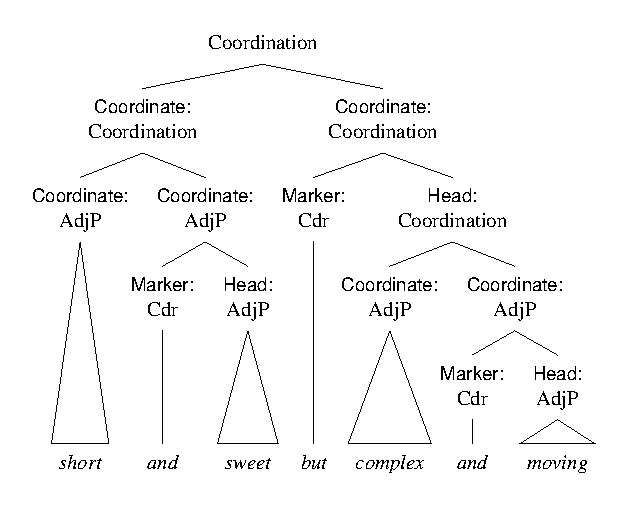
\includegraphics[width=0.9\linewidth]{figures/short and sweet but complex and moving.pdf}
    \caption{층위가 있는 등위접속: \mention{short and sweet but complex and moving}}\label{fig:coord-layered-ko}
\end{figure}

\subsection{특수한 등위접속}

특히 흥미로운 등위접속 유형은 비교 구조에 나타납니다.

\ea \label{ex:coord-comp-ko}
    \ea \gll He's as tall as {\ob}or taller than{\cb} his brother.\\
        he-이다 as 키-큰 as or 더-키-큰 than his 형제\\
    \glt \trans{그는 자기 형제만큼 키가 크거나 그보다 더 크다.}
    \ex \gll She writes more {\ob}but understands less{\cb} than before.\\
        she 쓰다-PRS 더-많이 but 이해하다-PRS 더-적게 than 이전\\
    \glt \trans{그녀는 이전보다 더 많이 쓰지만 더 적게 이해한다.}
    \z
\z
이 구조들에는 등위 요소와 그 요소들이 공유하는 성분 사이에 복잡한 관계가 포함되는 경우가 많습니다. 이를 해석하려면 등위접속과 비교 관계를 모두 이해해야 합니다.

\begin{tblsframedsymbol}{빠른 자기 점검: 복잡한 구조}{test}
층위가 있는 구조를 분석할 수 있는지 확인해 보십시오.
\begin{itemize}[noitemsep, leftmargin=*]
    \item \mention{I know that she left and he stayed}에서 모든 종속화 관계와 등위접속 관계를 찾으십시오.
    \item \mention{Both young and talented, she succeeded}에서 상관적 표지와 등위접속된 형용사를 찾으십시오.
    \item 다음 구조를 분석하십시오: \mention{He's taller than I thought but shorter than his brother}.
\end{itemize}
이 복잡한 유형들을 이해하면 종속화와 등위접속이 어떻게 함께 의미를 만드는지 볼 수 있습니다.
\end{tblsframedsymbol}

\section{정리}

종속화와 등위접속은 둘 다 생각을 잇는다는 같은 일을 하지만, 정반대의 구조를 사용합니다. 종속화는 삽입하고, 등위접속은 결합합니다. 좋은 글은 이 둘의 균형을 잡습니다. 학생이 어떤 구조를 만들려는지, 그리고 어디에서 그 구조가 어긋나는지를 알면 단순히 \enquote{뭔가 이상하다}고 느끼는 데서 그치지 않고 문제에 이름을 붙일 수 있습니다. 층이 너무 많다, 나열이 너무 많다, 등위접속사로 충분한 곳에 종속 접속사를 썼다, 이런 식으로 말입니다.

\end{document}
